%%%% h2snn_ijcai27.tex -- IJCAI-27 version of H2S-NN (rewritten from h2snn_manuscript.tex)
%%%% Experiments are unfinished: every number that does not exist yet is \res.

\documentclass{article}
\pdfpagewidth=8.5in
\pdfpageheight=11in

\usepackage{ijcai27}

\usepackage{times}
\usepackage{soul}
\usepackage{url}
\usepackage[hidelinks]{hyperref}
\usepackage[utf8]{inputenc}
\usepackage[small]{caption}
\usepackage{graphicx}
\usepackage{amsmath}
\usepackage{amssymb}
\usepackage{amsthm}
\usepackage{booktabs}
\usepackage{multirow}
\usepackage{algorithm}
\usepackage{algorithmic}
\usepackage[switch]{lineno}

% Comment out this line in the camera-ready submission
\linenumbers

\urlstyle{same}

\newtheorem{proposition}{Proposition}

\newcommand{\R}{\mathbb{R}}
\newcommand{\method}{\textsc{H2S-NN}}
\newcommand{\wisp}{\textsc{WISP}}
\newcommand{\norm}[1]{\left\lVert #1\right\rVert}
\newcommand{\transpose}{\mathsf{T}}
\newcommand{\concat}{\mathbin\Vert}
\newcommand{\res}{{\scriptsize[result]}}
\newcommand{\inc}{\trianglelefteq}

\pdfinfo{
/TemplateVersion (IJCAI.2027.0)
}

\title{H2S-NN: Heterogeneous Heterophilic Sheaf Neural Network with Path Instances}

% Anonymous submission
\author{
    Anonymous submission
}

\begin{document}

\maketitle

\begin{abstract}
In a heterogeneous graph, nodes and relations have several types; under heterophily, connected nodes often differ in label or features, so averaging neighbours is unreliable. Meta-paths such as paper--author--paper describe how two nodes are related through intermediate nodes. Existing methods use them either by splitting the graph into one homogeneous graph per meta-path, which removes the intermediate nodes from the computation, or by encoding each path instance into a feature of its target node only. We ask whether path instances can instead act inside the original graph. We propose the Heterogeneous Heterophilic Sheaf Neural Network with Path Instances (\method{}), a sheaf neural network on the original heterogeneous graph: each edge has learned maps that transform a message between its endpoints, so neighbours need not agree directly. Path instances are sampled by random walks without a meta-path list; each receives a weight computed from its own nodes and relation sequence, and every node of the instance, including intermediate nodes, receives its message through the same edge maps the graph uses. Edge and instance terms form one normalized operator, stable for any parameter values, to which a learned spectral filter is applied. On node-classification benchmarks spanning a range of heterophily, \res{}; ablations on identical sampled instances show \res{}.
\end{abstract}

%======================================================================
\section{Introduction}
\label{sec:introduction}

Heterogeneous graphs are a common representation for modeling complex relational structures, such as citation networks \cite{liu2014meta} or social interactions \cite{singh2025overview}. Unlike homogeneous graphs, heterogeneous graphs contain multiple types of nodes and relations with distinct semantic roles \cite{sun2013mining}. Moreover, many graphs are also heterophilic, meaning that adjacent nodes may have different labels or attributes, which makes similarity-based neighbor aggregation unreliable. A graph can be both heterogeneous and heterophilic \cite{lin2025heterophily}; in Figure~\ref{fig:example}(a), papers P1 and P9 share the author A7 but belong to different fields. Modeling such graphs under the simplifying assumptions of homogeneity or homophily can obscure the relational patterns that distinguish their nodes and consequently degrade predictive performance \cite{lin2025heterophily}.

Meta-paths are the standard way to express typed multi-hop relations. A meta-path schema such as \texttt{Paper-Author-Paper} (PAP) describes a co-authorship relation that is contained in neither endpoint alone \cite{sun2011pathsim}, and a path instance such as P1--A7--P9 is one concrete walk that follows it. This raises the question that motivates this work: \emph{P1 and P9 are linked through the author A7 and through the subject S3; does it matter who A7 and S3 are, or is it enough to know that P1 and P9 are connected?}

\begin{figure*}[t]
  \centering
  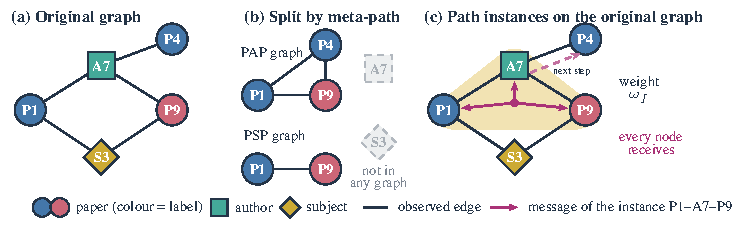
\includegraphics[width=0.92\textwidth]{figure/h2snn_example.pdf}
  \caption{Running example. \textbf{(a)} A heterogeneous heterophilic citation graph: papers P1, P4, P9 (colour = label), author A7, subject S3. \textbf{(b)} Splitting by meta-path builds one paper graph per schema (PAP, PSP); A7 and S3 appear in neither. \textbf{(c)} \method{} keeps the path instance P1--A7--P9 on the original graph: its message (arrows) reaches all three of its nodes, scaled by the instance weight $\omega_f$, and A7 passes it to P4 at the next step. The shaded region only marks the nodes of the instance.}
  \label{fig:example}
\end{figure*}

Existing methods answer this question in different ways. Most methods for heterogeneous heterophilic graphs split the graph by meta-path schema into latent or induced homogeneous graphs \cite{lu2026addressing,chen2025adaptive,li2025hetero2net,guo2023homophily,shen2025heterophily,wang2025homophily}, or precompute neighbour averages per schema \cite{yang2023sehgnn,li2024lmsps}. As Figure~\ref{fig:example}(b) shows, the intermediate nodes A7 and S3 then no longer take part in the computation. Instance encoders such as MAGNN \cite{fu2020magnn}, MECCH \cite{fu2024mecch}, and MF2Vec \cite{kim2024mf2vec} do keep the intermediate nodes: they encode each instance and aggregate the result into its target node. However, the encoding is written only to the target, and each schema is processed in its own subgraph, so A7 itself never learns about the pair (P1,~P9). Sheaf neural networks handle heterophily by comparing neighbours only after a learned transformation \cite{hansen2020sheaf,bodnar2022neural}, and HetSheaf applies them to the original heterogeneous graph \cite{braithwaite2024heterogeneous}, but only edges enter its operator. Finally, a recent study shows that a tuned R-GCN matches or outperforms many heterogeneous graph neural networks \cite{yang2025causal}, so a new component must be justified by controlled comparisons rather than by benchmark rankings alone.

To address this gap, we introduce the \textbf{Heterogeneous Heterophilic Sheaf Neural Network with Path Instances (\method{})}. \method{} works on the original graph. Each edge carries learned maps that transform a message from one endpoint into the space of the other, so neighbours need not agree directly. Path instances are sampled by random walks; each adds one term to the same operator, in which the nodes of the instance are compared after transport along the path, and every node of the instance, not only its end node, receives the correction (Figure~\ref{fig:example}(c)).
Our main contributions are summarized as follows:
\begin{enumerate}
  \item We let path instances act inside the propagation operator of the original heterogeneous graph: each instance is weighted individually from its own nodes and relations, and every node of the instance, including intermediate nodes, receives the instance's message, transformed by the same edge maps the graph uses.
  \item We develop Walk-sampled, Instance-weighted Sheaf Paths (\wisp{}), a sampler that draws path instances by random walks from a stated distribution with unbiased weights, so the model needs no meta-path list and no per-meta-path parameters, and its cost does not grow with the number of schemas.
  \item We design an evaluation that isolates each design choice on identical sampled instances: no instances, endpoint-only weights, free path maps, endpoint shortcut edges, and a naive combination of MAGNN-style instance features with an edge-only sheaf model; known-answer tasks are reported, including the one that failed.
\end{enumerate}

%======================================================================
\section{Preliminaries}
\label{sec:background}

\subsection{Heterogeneous Graphs}
A heterogeneous graph is a tuple $G=(V,E,\phi,\psi)$, where $V$ and $E$ are the node and edge sets, $\phi:V\rightarrow\mathcal{T}$ assigns each node a type, and $\psi:E\rightarrow\mathcal{R}$ assigns each edge a relation type. The graph is heterogeneous when $|\mathcal{T}|>1$ or $|\mathcal{R}|>1$; it reduces to a homogeneous graph when $|\mathcal{T}|=|\mathcal{R}|=1$ \cite{lu2026addressing}. Benchmarks often store each fact twice, once per direction; we keep one oriented edge per fact.

\subsection{Meta-Path Schemas and Path Instances}
A meta-path schema of length $\ell$ is a typed relation sequence
\begin{equation}
  \pi:\;
  t_0 \xrightarrow{r_1} t_1 \xrightarrow{r_2}\cdots
  \xrightarrow{r_\ell} t_\ell,
  \qquad t_i\in\mathcal{T},\; r_i\in\mathcal{R},
  \label{eq:schema}
\end{equation}
which specifies a composite relation between its endpoint types \cite{sun2011pathsim}. A path instance is an ordered sequence $f=(v_0,e_1,v_1,\ldots,e_\ell,v_\ell)$ of nodes and edges with $\phi(v_i)=t_i$ and $\psi(e_i)=r_i$. Thus, $\pi$ describes a type-level pattern, whereas $f$ identifies one occurrence of that pattern in the observed graph; we call $v_1,\ldots,v_{\ell-1}$ the intermediate nodes of $f$. For example, PAP is a schema and P1--A7--P9 is one of its instances, with A7 as its intermediate node.

\subsection{Homophily and Heterophily}
Homophily refers to the prevalence of edges between nodes that share the same label. In a heterogeneous graph, labels are usually comparable only between nodes of the target type, so heterophily is measured on the graphs induced by meta-paths. Let $\mathcal{P}_2$ be the set of length-two schemas from the target type to itself and $G_p$ the graph that $p\in\mathcal{P}_2$ induces on target nodes. We report two measures exactly as their sources define and implement them. The primary measure is the $\mathcal{H}^2$ index of H2GB \cite{lin2025heterophily},
\begin{equation}
  \mathcal{H}^2(G)=\frac{1}{|\mathcal{P}_2|}\sum_{p\in\mathcal{P}_2}\bigl(1-h_{\mathrm{adj}}(G_p)\bigr),
  \label{eq:h2}
\end{equation}
where $h_{\mathrm{adj}}$ is the adjusted homophily of Platonov et al.~\shortcite{platonov2023characterizing}, which corrects edge homophily for class imbalance. Values near $0$ indicate homophily, and values near or above $1$ indicate heterophily. Next to it we report the metapath-based label heterophily (MLH) \cite{li2025hetero2net}, which averages the uncorrected edge heterophily over the same graphs.

\subsection{Cellular Sheaves on Graphs}
A cellular sheaf $\mathcal{F}$ on a graph assigns a vector space, or \emph{stalk}, to every node and edge, and a linear restriction map $F_{v\inc e}:\mathcal{F}(v)\rightarrow\mathcal{F}(e)$ to every incident pair. We call these maps \emph{edge maps}: $F_{v\inc e}$ expresses the state of node $v$ in the space of edge $e$. With $d$-dimensional stalks, the coboundary compares the two endpoints of an oriented edge $e=(u\rightarrow v)$ after both are mapped into the edge stalk:
\begin{equation}
  (\delta x)_e = F_{v\inc e}x_v-F_{u\inc e}x_u .
  \label{eq:coboundary}
\end{equation}
The sheaf Laplacian $\Delta_0=\delta^{\transpose}\delta$ has energy $x^{\transpose}\Delta_0x=\norm{\delta x}^2$; when all maps are identities, it recovers the graph Laplacian. Sheaf neural networks can address heterophily and oversmoothing by diffusing through learned edge maps instead of averaging raw features \cite{hansen2020sheaf,bodnar2022neural}, which has led to numerous extensions \cite{barbero2022sheaf,fiorini2025sheaves,ribeiro2026cooperative}, including HetSheaf for heterogeneous graphs \cite{braithwaite2024heterogeneous}. These models define the sheaf only over node--edge incidences.

%======================================================================
\section{Methodology}
\label{sec:method}

\subsection{Problem Formulation}
We consider supervised prediction on a heterogeneous graph $G=(V,E,\phi,\psi,X^{\mathrm{raw}})$ in which neighboring nodes may have different labels or features. Here, $X^{\mathrm{raw}}=\{x_v^{\mathrm{raw}}\}_{v\in V}$ contains type-dependent node features with $x_v^{\mathrm{raw}}\in\R^{d_{\phi(v)}}$; node types without features receive a learned vector per node. Unlike meta-path methods, the model is given no list of meta-path schemas: path instances are drawn by the model itself (Section~\ref{sec:wisp}). The learning problem is to construct a predictor $\hat{y}_o=g_\theta(o;G)$ for a supervised object $o$, which is a target node for node classification, a typed node pair for link prediction, and a graph for graph classification. Given labeled training objects $\mathcal{S}_{\mathrm{train}}$, the parameters are learned by minimizing
\begin{equation}
  \min_\theta\;
  \frac{1}{|\mathcal{S}_{\mathrm{train}}|}
  \sum_{o\in\mathcal{S}_{\mathrm{train}}}
  \mathcal{L}\bigl(g_\theta(o;G),y_o\bigr),
  \label{eq:objective}
\end{equation}
where $\mathcal{L}$ is cross-entropy for single-label targets and binary cross-entropy for multilabel targets and link prediction.

\subsection{Overview}
As shown in Figure~\ref{fig:pipeline}, \method{} consists of six steps. First, \emph{node encoding} maps typed features into a shared $d$-dimensional stalk space and adds a summary of each node's neighbours. Second, \emph{edge maps} define a sheaf on the original graph. Third, \wisp{} samples path instances by random walks, and fourth, each instance receives a learned weight. Fifth, every instance adds an \emph{instance term} that compares its nodes after transport along the path. Finally, edge and instance terms form one normalized operator, to which a gated Chebyshev filter bank is applied before a prediction head. The edge maps, gates, and instance weights are computed once per forward pass from the encoded nodes, so all propagation acts on one sheaf.

\begin{figure*}[t]
  \centering
  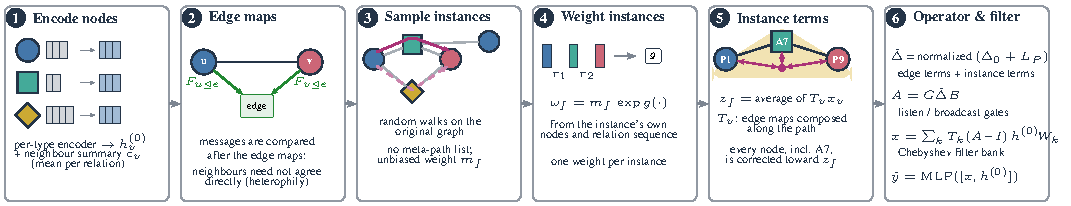
\includegraphics[width=\textwidth]{figure/h2snn_overview_v2.pdf}
  \caption{Overview of \method{}. \textbf{(1)} Type-specific encoders map node features to a common $d$-dimensional stalk; a parameter-free summary $c_v$ of each node's neighbours is added. \textbf{(2)} Each edge has learned maps $F_{u\inc e},F_{v\inc e}$; endpoint messages are compared only after these maps. \textbf{(3)} \wisp{} samples path instances by random walks on the original graph, without a meta-path list, with an unbiased weight $m_f$. \textbf{(4)} Each instance receives a weight $\omega_f$ from its own nodes and relation sequence. \textbf{(5)} The nodes of an instance are transported along the path with the edge maps, compared with their average $z_f$, and all of them are corrected, including the intermediate node A7. \textbf{(6)} Edge and instance terms form one normalized operator, filtered with listen/broadcast gates and a Chebyshev filter bank; a head reads $[x,h^{(0)}]$.}
  \label{fig:pipeline}
\end{figure*}

\subsection{Node Encoding and Neighbourhood Summary}
\method{} first maps type-dependent node features into a shared $d$-dimensional stalk space, so that nodes of different types can be compared by the same edge maps. For each node $v$, we compute
\begin{equation}
  h_v^{(0)}=\operatorname{GELU}\!\left(\operatorname{LN}\!\left(W_{\phi(v)}x_v^{\mathrm{raw}}+b_{\phi(v)}\right)+q_{\phi(v)}\right)\in\R^{d},
  \label{eq:encoder}
\end{equation}
where $W_t$ and $b_t$ are type-specific parameters and $q_t$ is a learned type embedding. Two nodes with similar features can still play different relational roles, for example a prolific and a junior author. We therefore add a parameter-free summary of each node's typed neighbourhood: for every relation type $r$ and role $\rho\in\{\mathrm{src},\mathrm{tgt}\}$, $c_v$ concatenates the mean of $h^{(0)}$ over the neighbours of $v$ under $(r,\rho)$. The edge maps and gates below read $[h_v^{(0)},c_v]$; they are computed once, so the geometry does not change during propagation.

\subsection{Edge Maps: a Sheaf on the Original Graph}
Each edge transforms messages between its endpoints, so that heterophilic neighbours are compared after a learned change of coordinates rather than directly. For an oriented edge $e=(u\xrightarrow{r}v)$, the edge maps are
\begin{equation}
  F_{u\inc e}=\lambda_e R_{r,\mathrm{src}}H_{u,e},\qquad
  F_{v\inc e}=\lambda_e R_{r,\mathrm{tgt}}H_{v,e},
  \label{eq:edge-maps}
\end{equation}
where $R_{r,\rho}\in SO(d)$ is a learned frame for relation $r$ and role $\rho$, $H_{z,e}$ is a product of $k$ Householder reflections whose vectors are predicted from $[h_u^{(0)},c_u]$, $[h_v^{(0)},c_v]$, the relation embedding $\zeta_r$ and the role of $z$, and $\lambda_e>0$ is one scale per edge. Thus, the maps depend on the relation, on the direction of the edge and on both endpoints, and every map is a positive multiple of an orthogonal matrix. The node operator over edges is the sheaf Laplacian $\Delta_0$ of Equation~\eqref{eq:coboundary}. Because the two maps of an edge share one scale, the scale cancels when a message crosses the edge, and every composition of edge maps along a path is orthogonal.

\subsection{\wisp{}: Schema-Free Sampling of Path Instances}
\label{sec:wisp}
\wisp{} answers which path instances can enter the model without a meta-path list. From every node of the target type (the \emph{anchor}), it draws $r$ random walks on the original graph. A walk first draws its length $\ell$ uniformly from $\{2,\ldots,\ell_{\max}\}$; at each hop it chooses uniformly among the available relation--direction pairs that still lead to an unvisited node, and then chooses uniformly among those neighbours. A walk that reaches a dead end before its length is discarded. This defines a probability $p(\omega\mid a)$ for every simple walk $\omega$ from anchor $a$, and the operator that the instances are meant to represent,
\begin{equation}
  L_P^{\mathrm{target}}=\sum_{a}\sum_{\omega}p(\omega\mid a)\,L_{f(\omega)},
  \label{eq:target}
\end{equation}
where $f(\omega)$ is the instance traced by $\omega$ and $L_f$ is its instance term (Section~\ref{sec:instance-term}). Walks may be drawn from a mixture $\tfrac12p+\tfrac12q$ with any proposal $q$, and each instance receives the importance weight
\begin{equation}
  m_f=\sum_{\omega\rightarrow f}\frac{1}{r}\,\frac{p(\omega)}{\tfrac12p(\omega)+\tfrac12q(\omega)},
  \label{eq:mf}
\end{equation}
summed over the sampled walks that trace $f$; a path and its reversal are one instance. Each walk contributes at most $2/r$, whatever its length. With these weights, $\mathbb{E}[\sum_f m_fL_f]=L_P^{\mathrm{target}}$ for every proposal (Appendix~\ref{app:proofs}); our experiments use $q=p$. Training draws new walks every epoch, and evaluation uses one fixed draw, so every compared model sees the same evaluation instances. The schema of an instance (e.g., PAP) is a label read from the walk, not an input. Hence, the number of candidate schemas does not enter the cost, and the share of instance weight per schema can be reported after training.

\subsection{Instance Weights}
Instances of the same schema can carry different information: a PAP instance through a prolific, off-topic author may deserve less trust than another PAP instance. Each instance therefore receives its own positive weight,
\begin{equation}
\begin{aligned}
  \omega_f&=m_f\exp\!\bigl(g(\xi_f)\bigr),\\
  \xi_f&=\bigl[h_{v_0}^{(0)}\concat\cdots\concat h_{v_\ell}^{(0)}\concat\zeta_{r_1}\concat\cdots\concat\zeta_{r_\ell}\bigr],
\end{aligned}
  \label{eq:weight}
\end{equation}
where $g$ is a small network for each path length that reads every node of the instance in path order and its relation sequence. The weight corrects the sampling through $m_f$ and scores the instance through $g$. The input $\xi_f$ uses $h^{(0)}$ and not the neighbourhood summary $c$, so that a variant whose $g$ reads only the endpoints indeed has no access to the intermediate nodes. Uniform weights, schema-only weights and endpoint-only weights are restrictions of Equation~\eqref{eq:weight}, which we use as controls in Section~\ref{sec:discussion}.

\subsection{Instance Terms}
\label{sec:instance-term}
Each instance adds one term to the operator, which asks all of its nodes to agree after transport along the path. For an instance $f=(v_0,e_1,v_1,\ldots,e_\ell,v_\ell)$, the transport brings the stalk of every node of $f$ into the frame of $v_0$ by composing the edge maps along the path:
\begin{equation}
  T_{v_0}=I,\qquad
  T_{v_i}=T_{v_{i-1}}F_{v_{i-1}\inc e_i}^{-1}F_{v_i\inc e_i},\quad i=1,\ldots,\ell .
  \label{eq:transport}
\end{equation}
Here, $F_{v_i\inc e_i}x_{v_i}$ expresses $x_{v_i}$ in the space of the edge $e_i$, the inverse map returns it to the frame of $v_{i-1}$, and $T_{v_{i-1}}$ continues to $v_0$. The transports are therefore not free parameters: they are fixed by the edge maps of the instance's own edges. The instance term then compares each transported state with the average of the instance,
\begin{equation}
\begin{aligned}
  z_f&=\frac{1}{\ell+1}\sum_{v\in f}T_vx_v,\\
  x^{\transpose}L_Px&=\sum_f\omega_f\sum_{v\in f}\norm{T_vx_v-z_f}^2 .
\end{aligned}
  \label{eq:instance-term}
\end{equation}
For P1--A7--P9, $z_f$ averages the three transported states, and the gradient of the term moves P1, A7, and P9 toward $z_f$; hence the intermediate node A7 receives the message of the instance and, through its edge to P4, passes it on at the next application of the operator.

Three properties follow directly. First, an instance never contradicts the edges: if $\delta x=0$, then $F_{v_{i-1}\inc e_i}x_{v_{i-1}}=F_{v_i\inc e_i}x_{v_i}$ on every edge of $f$, so all $T_vx_v$ are equal and the term vanishes; adding instances keeps every state that the edges already accept. Second, computationally an instance term is equivalent to one additional hub node joined to every node of the instance, with the transports $T_v$ as its edge maps and the hub state eliminated, because the minimizer of $\sum_v\norm{T_vx_v-z}^2$ over $z$ is $z_f$ (Appendix~\ref{app:proofs}, Prop.~2). Third, if the edge maps depended only on the relation type, $z_f$ would coincide with the relational rotation encoder of MAGNN \cite{fu2020magnn}. \method{} differs in that its maps depend on both endpoints, are the same maps the edges use, and return the message to every node of the instance rather than to the target alone.

\subsection{Operator, Gates, and Filter}
Edge terms and instance terms form one operator. To keep it stable for any learned parameters, we normalize it by its block-diagonal degree $D$:
\begin{equation}
  \hat{\Delta}=D^{-1/2}\bigl(\Delta_0+L_P\bigr)D^{-1/2}.
  \label{eq:operator}
\end{equation}
Because every edge and instance term $L$ satisfies $L\preceq 2D_L$ for its own degree, the spectrum of $\hat{\Delta}$ lies in $[0,2]$ for every value of the parameters (Appendix~\ref{app:proofs}, Prop.~3). Under heterophily, influence need not be symmetric: a subject shared by thousands of papers should inform them without being pulled toward each one. We therefore add a listen gate $\gamma_u\in(0,1)$ and a broadcast gate $\beta_v\in(0,1)$ per node, read from $[h^{(0)},c]$, and use $A=\Gamma\hat{\Delta}B$ with $\Gamma=\operatorname{diag}(\gamma)$ and $B=\operatorname{diag}(\beta)$. The influence of $v$ on $u$ is thus scaled by $\gamma_u\beta_v$: if $\gamma_u=0$, node $u$ ignores the others, and if $\beta_v=0$, node $v$ influences no one. $A$ is self-adjoint in the node metric $B\Gamma^{-1}$, so its spectrum is real and lies in $[0,2)$.

Part of the label signal under heterophily lies in disagreement between transported neighbours, that is, in high and middle frequencies of the operator, which repeated first-order diffusion only damps. We therefore apply a Chebyshev filter bank \cite{defferrard2016chebnet,he2022chebnetii} with a separate response per stalk coordinate:
\begin{equation}
  x=\sum_{k=0}^{K}C_k(A-I)\,h^{(0)}W_k,\qquad \sum_k\norm{W_k}_2\le 1,
  \label{eq:filter}
\end{equation}
where $C_k$ is the $k$-th Chebyshev polynomial and $W_k\in\R^{d\times d}$ mixes stalk coordinates within each frequency band. Since the spectrum of $A-I$ lies in $[-1,1)$, every $C_k(A-I)$ has norm at most one, and the filter has gain at most one for all parameter values (Appendix~\ref{app:proofs}, Prop.~5). Finally, the prediction for node $v$ is $\hat{y}_v=\operatorname{MLP}([x_v\concat h_v^{(0)}])$; keeping the node's own encoding separate from the propagated state avoids mixing a node with disagreeing neighbours before the nonlinear head \cite{zhu2020beyond}. Link prediction uses the same states with a pair decoder, and graph classification uses sum pooling (Appendix~\ref{app:heads}).

\paragraph{Complexity.} The edge maps are applied as one relation frame and $k$ reflections, so no $d\times d$ matrix is stored per edge. Each application of $A$ costs $O\bigl((|E|+I)(d^2+kd)\bigr)$, where $I$ is the number of node--instance incidences; the cost is linear in edges and incidences and does not depend on the number of schemas.

%======================================================================
\section{Experiments}
\label{sec:experiments}

\subsection{Experiment Settings}
To assess \method{} across heterogeneous graph learning settings, we evaluated it on node classification, the main task, and on link prediction; graph classification is reported in Appendix~\ref{app:data} as a check that the model covers the task.

\paragraph{Datasets.}
For node classification, we used four HGB benchmarks \cite{lv2021hgb}, ACM, DBLP, IMDB, and Freebase, and four H2GB benchmarks \cite{lin2025heterophily}, IEEE-CIS-G, mag-year, ogbn-mag, and H-Pokec, which together cover a wide range of heterophily (Table~\ref{tab:node-cls}). We computed $\mathcal{H}^2$ and MLH with the reference implementations; for IMDB, whose movies have several genres, the measures are averaged over the five binary genre labels. For link prediction, we derived tasks from the node-classification graphs, ACM paper--author, DBLP author--paper, IMDB movie--actor, and Freebase book--book, and used HGB PubMed and LastFM \cite{lv2021hgb}. In the link-prediction files, node features that are computed from the target relation or describe the other endpoint are removed, because they reveal held-out links. Dataset statistics are given in Appendix~\ref{app:data}.

\paragraph{Baselines.}
For node classification, we compared \method{} with baselines from four model categories. The homogeneous homophilic baselines comprised GCN \cite{kipf2017gcn}, GAT \cite{velickovic2018gat}, and ChebNetII \cite{he2022chebnetii}, while the homogeneous heterophilic baselines included NSD \cite{bodnar2022neural} and CSNN \cite{ribeiro2026cooperative}. For heterogeneous graphs, we considered the homophilic models R-GCN \cite{schlichtkrull2018rgcn}, HAN \cite{wang2019han}, MAGNN \cite{fu2020magnn}, SeHGNN \cite{yang2023sehgnn}, HiNormer \cite{mao2023hinormer}, and PSHGCN \cite{he2024spectral}, as well as the heterophilic models H2G-former \cite{lin2025heterophily}, Hetero$^2$Net \cite{li2025hetero2net}, H2SGNN \cite{lu2026addressing}, HetSheaf \cite{braithwaite2024heterogeneous}, and LatGRL \cite{shen2025heterophily}. For link prediction, we used a subset of these baselines while retaining representatives from all four categories.

\paragraph{Evaluation Settings.}
For node classification, we followed the official splits of HGB (24\%/6\%/70\%) and H2GB and reported Macro-F1 and Micro-F1 (H2GB datasets: the metric of the benchmark). IMDB is evaluated as five binary genre labels with a fixed threshold. For link prediction, the target relation was split by fact into 81\%/9\%/10\%, and every held-out fact was removed in both directions from the message graph and from every sampled instance. We reported MRR and Hits@10 against hard negatives for each positive, built as in HeaRT \cite{li2023heart} with candidates restricted to the endpoint type, separately for pairs whose endpoints are seen in training and for cold-start pairs. All methods, including every baseline, were rerun under one protocol with the same tuning budget, model selection on validation only, and ten seeds; we report means and standard deviations and test each comparison with a paired Wilcoxon test with Holm correction. The \wisp{} settings were fixed before any run and never tuned: $\ell_{\max}=4$ on HGB, and $r$ chosen so that the number of node--instance incidences matches that of the literature meta-paths on the same dataset. Following HGB \cite{lv2021hgb}, we group the baselines as Hom./hom., Hom./het., Het./hom., and Het./het., where the first term indicates whether the graph is modeled as homogeneous or heterogeneous and the second whether the method is designed for homophilic or heterophilic settings.

\subsection{Results}
\label{sec:results}

Table~\ref{tab:node-cls} reports node classification. \res{}

\begin{table*}[t]
  \centering
  \caption{Node classification (Macro-F1 for HGB; benchmark metric for H2GB), mean $\pm$ std over ten seeds. The second header row gives $\mathcal{H}^2$ (higher = more heterophilic). Best values are bold.}
  \label{tab:node-cls}
  \footnotesize
  \setlength{\tabcolsep}{4pt}
  \begin{tabular}{llcccccccc}
    \toprule
    & & ACM & DBLP & IMDB & Freebase & IEEE-CIS-G & mag-year & ogbn-mag & H-Pokec \\
    \textbf{Group} & \textbf{Model} & \res & \res & 0.737 & 0.995 & \res & \res & \res & \res \\
    \midrule
    \multirow{3}{*}{Hom./hom.} & GCN & \res & \res & \res & \res & \res & \res & \res & \res \\
    & GAT & \res & \res & \res & \res & \res & \res & \res & \res \\
    & ChebNetII & \res & \res & \res & \res & \res & \res & \res & \res \\
    \midrule
    \multirow{2}{*}{Hom./het.} & NSD & \res & \res & \res & \res & \res & \res & \res & \res \\
    & CSNN & \res & \res & \res & \res & \res & \res & \res & \res \\
    \midrule
    \multirow{6}{*}{Het./hom.} & R-GCN & \res & \res & \res & \res & \res & \res & \res & \res \\
    & HAN & \res & \res & \res & \res & \res & \res & \res & \res \\
    & MAGNN & \res & \res & \res & \res & \res & \res & \res & \res \\
    & SeHGNN & \res & \res & \res & \res & \res & \res & \res & \res \\
    & HiNormer & \res & \res & \res & \res & \res & \res & \res & \res \\
    & PSHGCN & \res & \res & \res & \res & \res & \res & \res & \res \\
    \midrule
    \multirow{5}{*}{Het./het.} & H2G-former & \res & \res & \res & \res & \res & \res & \res & \res \\
    & Hetero$^2$Net & \res & \res & \res & \res & \res & \res & \res & \res \\
    & H2SGNN & \res & \res & \res & \res & \res & \res & \res & \res \\
    & HetSheaf & \res & \res & \res & \res & \res & \res & \res & \res \\
    & LatGRL & \res & \res & \res & \res & \res & \res & \res & \res \\
    \midrule
    Ours & \method{} & \res & \res & \res & \res & \res & \res & \res & \res \\
    \bottomrule
  \end{tabular}
\end{table*}

Table~\ref{tab:link-pred} reports link prediction. \res{}

\begin{table}[t]
  \centering
  \caption{Link prediction, MRR with HeaRT hard negatives (mean over ten seeds). Hits@10, AUROC/AUPR, and the seen/cold-start split are in Appendix~\ref{app:data}.}
  \label{tab:link-pred}
  \footnotesize
  \setlength{\tabcolsep}{2.6pt}
  \begin{tabular}{lcccccc}
    \toprule
    \textbf{Model} & ACM & DBLP & IMDB & Freebase & PubMed & LastFM \\
    \midrule
    GCN & \res & \res & \res & \res & \res & \res \\
    NSD & \res & \res & \res & \res & \res & \res \\
    R-GCN & \res & \res & \res & \res & \res & \res \\
    MAGNN & \res & \res & \res & \res & \res & \res \\
    HetSheaf & \res & \res & \res & \res & \res & \res \\
    H2G-former & \res & \res & \res & \res & \res & \res \\
    \midrule
    \method{} & \res & \res & \res & \res & \res & \res \\
    \bottomrule
  \end{tabular}
\end{table}

%======================================================================
\section{Discussion}
\label{sec:discussion}

\subsection{Ablation Study: What the Instances Contribute}
To isolate the contribution of each design choice, we compared the full \method{} with variants that use the same sampled instances, the same evaluation draw, and parameter counts within 5\% (Table~\ref{tab:ablation}). \emph{No instances} removes $L_P$. The \emph{weight ladder} restricts $g$ in Equation~\eqref{eq:weight} to a constant (uniform), to the relation sequence (schema), or to the endpoints and relation sequence (endpoints); the full model differs from the endpoints variant only in seeing the intermediate nodes. \emph{Endpoint shortcut} replaces each instance by one edge between its endpoints carrying the composed transport, which is what eliminating the intermediate nodes leaves (Appendix~\ref{app:proofs}) and what a closure edge between the endpoints computes. \emph{Free path maps} replaces the transports by freely learned maps per node and instance, as in sheaf hypergraph networks \cite{duta2023sheafhyper}. The \emph{naive combination} encodes the same instances with MAGNN's rotation encoder and instance attention and feeds them as node features to the model without instances, which tests whether joining the two ideas inside one operator adds anything over placing them side by side. The criterion was fixed before running: if the full model is not significantly better than the endpoints variant on at least two of ACM, DBLP, and IMDB, we do not claim that the intermediate nodes contribute through the instance weights. \res{}

\begin{table}[t]
  \centering
  \caption{Ablations on identical sampled instances (Macro-F1, mean over ten seeds; $^\dagger$: significantly below the full model, paired Wilcoxon with Holm correction).}
  \label{tab:ablation}
  \footnotesize
  \setlength{\tabcolsep}{3pt}
  \begin{tabular}{lcccc}
    \toprule
    \textbf{Variant} & ACM & DBLP & IMDB & Freebase \\
    \midrule
    \method{} (full) & \res & \res & \res & \res \\
    No instances & \res & \res & \res & \res \\
    Uniform weights & \res & \res & \res & \res \\
    Schema weights & \res & \res & \res & \res \\
    Endpoint weights & \res & \res & \res & \res \\
    Endpoint shortcut & \res & \res & \res & \res \\
    Free path maps & \res & \res & \res & \res \\
    Naive combination & \res & \res & \res & \res \\
    Encoder only ($h^{(0)}$) & \res & \res & \res & \res \\
    \bottomrule
  \end{tabular}
\end{table}

\subsection{Known-Answer Tasks}
Benchmark accuracy cannot show whether the instance weights learn what they are meant to learn, so we also report synthetic tasks whose answer is known. In S1$'$, the label of each target is carried by one decisive instance among many instances of the same schema. When the decisive instances were up-weighted by a fixed factor of 512 and only a common bias was learned, the model reached test accuracies of 0.992, 0.988, and 0.996 on three seeds, whereas equal weights stayed at chance; the operator can therefore use correct instance weights. However, the full model did not learn them: all instance weights rose together and no selection emerged. Two further tasks, S3 (instance-level selection) and S2$'$ (recovering a planted long schema), are run with the main protocol. \res{}

\subsection{Limitations}
The weights scale how strongly an instance acts but cannot change its transports, which are fixed by its edges; instances are simple walks, so branching meta-structures are not represented; and the ratio of influence in the two directions of a pair is determined by the two nodes' gates. On the largest graphs, training uses local subgraphs around target nodes, which approximates the full operator outside each subgraph.

%======================================================================
\section{Conclusion}
To address heterogeneous graph learning under heterophily, we proposed \method{}, a sheaf neural network in which path instances act inside the operator of the original heterogeneous graph. Each instance is sampled without a meta-path list, weighted from its own nodes and relations, and compared through the same edge maps that the graph uses, so that its intermediate nodes receive its message instead of disappearing into a meta-path graph. \res{}

\bibliographystyle{named}
\bibliography{references}

%======================================================================
% Supplementary appendix (to be moved to the separate supplementary file at submission)
\appendix
\section{Proofs}
\label{app:proofs}
Throughout, every edge map is $\lambda_e$ times an orthogonal matrix, with the same $\lambda_e$ on both sides of an edge, so every transport $T_v$ in Equation~\eqref{eq:transport} is orthogonal.

\begin{proposition}[Unbiased instances]
For walks drawn independently, $r$ per anchor, from $\tfrac12p+\tfrac12q$, $\mathbb{E}\bigl[\sum_f m_fL_f\bigr]=L_P^{\mathrm{target}}$, and each walk contributes at most $2/r$ to $m_f$.
\end{proposition}
\begin{proof}
By linearity, $\mathbb{E}[\sum_fm_fL_f]=\sum_a r\sum_\omega(\tfrac12p+\tfrac12q)(\omega)\,\tfrac1r\,\tfrac{p(\omega)}{\frac12p(\omega)+\frac12q(\omega)}L_{f(\omega)}=\sum_a\sum_\omega p(\omega)L_{f(\omega)}$. The ratio $p/(\tfrac12p+\tfrac12q)$ is at most $2$.
\end{proof}

\begin{proposition}[Hub-node equivalence]
Join a hub node $z_f$ to every node $v$ of $f$ by an edge whose maps are $T_v$ on the side of $v$ and $I$ on the side of the hub. Eliminating the hub state from the energy $\omega_f\sum_{v\in f}\norm{T_vx_v-z_f}^2$ gives exactly the instance term of Equation~\eqref{eq:instance-term}.
\end{proposition}
\begin{proof}
For fixed $x$, the energy is a convex quadratic in $z_f$ with minimizer $\frac{1}{\ell+1}\sum_vT_vx_v$; substituting it gives Equation~\eqref{eq:instance-term}, which is the Schur complement of the star Laplacian with respect to the hub.
\end{proof}

\begin{proposition}[Bounded operator]
$\Delta_0+L_P\preceq 2D$, where $D$ is its block diagonal; hence the spectrum of $\hat{\Delta}$ lies in $[0,2]$ for all parameter values.
\end{proposition}
\begin{proof}
For an edge, $\norm{F_{v\inc e}x_v-F_{u\inc e}x_u}^2\le2\lambda_e^2(\norm{x_u}^2+\norm{x_v}^2)$, and $\lambda_e^2I$ is the diagonal block that the edge adds at $u$ and at $v$. For an instance with $n=\ell+1\ge3$ nodes and $y_v=T_vx_v$, $\sum_v\norm{y_v-\bar y}^2\le\sum_v\norm{y_v}^2=\sum_v\norm{x_v}^2\le2(1-\tfrac1n)\sum_v\norm{x_v}^2$, and $\omega_f(1-\frac1n)I$ is the diagonal block that the instance adds at each of its nodes. Summing over all terms gives the claim.
\end{proof}

\begin{proposition}[Endpoint shortcut]
If the intermediate nodes of $f$ are eliminated from $\omega_f\sum_v\norm{T_vx_v-z_f}^2$, the result is $\frac{\omega_f}{2}\norm{T_{v_0}x_{v_0}-T_{v_\ell}x_{v_\ell}}^2$, an edge between the endpoints whose transport is the composition along the path and whose weight does not depend on any intermediate node.
\end{proposition}
\begin{proof}
With $y_v=T_vx_v$ and orthogonal $T_v$, the intermediate $y_v$ are free; the minimum of $\sum_v\norm{y_v-\bar y}^2$ over them sets every intermediate $y_v$ to $\frac12(y_{v_0}+y_{v_\ell})$, which leaves $\frac12\norm{y_{v_0}-y_{v_\ell}}^2$.
\end{proof}

\begin{proposition}[Filter gain]
For all parameter values, the spectrum of $A=\Gamma\hat{\Delta}B$ is real and lies in $[0,2\max_v\gamma_v\beta_v]\subset[0,2)$, and the filter of Equation~\eqref{eq:filter} has gain at most $\sum_k\norm{W_k}_2\le1$ in the norm induced by $M=B\Gamma^{-1}$.
\end{proposition}
\begin{proof}
$A$ is similar to $(\Gamma B)^{1/2}\hat{\Delta}(\Gamma B)^{1/2}$, which is symmetric, positive semidefinite, and bounded by $2\max_v\gamma_v\beta_v$; moreover $MA=B\hat{\Delta}B$ is symmetric, so $A$ is self-adjoint in $\langle\cdot,M\cdot\rangle$. Hence the spectrum of $A-I$ lies in $[-1,1)$ and $\norm{C_k(A-I)}_M\le1$. Because $M$ acts on each node by a scalar, it commutes with the per-node map $W_k$, whose $M$-norm is $\norm{W_k}_2$.
\end{proof}

\section{Prediction Heads}
\label{app:heads}
For node classification, $\hat{y}_v=\operatorname{MLP}([x_v\concat h_v^{(0)}])$. For link prediction, both endpoints use $z_v=[x_v\concat h_v^{(0)}]$ and a relation-specific bilinear decoder scores the pair. For graph classification, node states are summed over the graph and passed to an MLP; sum pooling is permutation invariant and can distinguish multisets \cite{xu2019gin}.

\section{Datasets, Settings, and Full Results}
\label{app:data}
Dataset statistics (nodes, facts, node and relation types, labelled targets, $\mathcal{H}^2$ and MLH per dataset and per genre for IMDB), the tuning budget and search spaces, the \wisp{} settings per dataset, link-prediction results with Hits@10, AUROC and AUPR and the seen/cold-start split, and graph classification on MUTAG, PROTEINS, ENZYMES, and NCI1 (atom and bond labels read as node and relation types) are reported here. \res{}

\end{document}
